%%
%% This is file `sample-sigconf.tex',
%% generated with the docstrip utility.
%%
%% The original source files were:
%%
%% samples.dtx  (with options: `sigconf')
%% 
%% IMPORTANT NOTICE:
%% 
%% For the copyright see the source file.
%% 
%% Any modified versions of this file must be renamed
%% with new filenames distinct from sample-sigconf.tex.
%% 
%% For distribution of the original source see the terms
%% for copying and modification in the file samples.dtx.
%% 
%% This generated file may be distributed as long as the
%% original source files, as listed above, are part of the
%% same distribution. (The sources need not necessarily be
%% in the same archive or directory.)
%%
%% Commands for TeXCount
%TC:macro \cite [option:text,text]
%TC:macro \citep [option:text,text]
%TC:macro \citet [option:text,text]
%TC:envir table 0 1
%TC:envir table* 0 1
%TC:envir tabular [ignore] word
%TC:envir displaymath 0 word
%TC:envir math 0 word
%TC:envir comment 0 0
%%


%%
%% The first command in your LaTeX source must be the \documentclass command.
\documentclass[sigconf]{acmart}

 

%% NOTE that a single column version may be required for 
%% submission and peer review. This can be done by changing
%% the \doucmentclass[...]{acmart} in this template to 
%% \documentclass[manuscript,screen]{acmart}
%% 
%% To ensure 100% compatibility, please check the white list of
%% approved LaTeX packages to be used with the Master Article Template at
%% https://www.acm.org/publications/taps/whitelist-of-latex-packages 
%% before creating your document. The white list page provides 
%% information on how to submit additional LaTeX packages for 
%% review and adoption.
%% Fonts used in the template cannot be substituted; margin 
%% adjustments are not allowed.
%%
%%
%% \BibTeX command to typeset BibTeX logo in the docs
\AtBeginDocument{%
  \providecommand\BibTeX{{%
    \normalfont B\kern-0.5em{\scshape i\kern-0.25em b}\kern-0.8em\TeX}}}

%% Rights management information.  This information is sent to you
%% when you complete the rights form.  These commands have SAMPLE
%% values in them; it is your responsibility as an author to replace
%% the commands and values with those provided to you when you
%% complete the rights form.
\copyrightyear{2023} 
\acmYear{2023} 
\setcopyright{acmlicensed}\acmConference[ICAIF '23]{4th ACM International Conference on AI in Finance}{November 27--29, 2023}{Brooklyn, NY, USA}
\acmBooktitle{4th ACM International Conference on AI in Finance (ICAIF '23), November 27--29, 2023, Brooklyn, NY, USA}
\acmPrice{15.00}
\acmDOI{10.1145/3604237.3626838}
\acmISBN{979-8-4007-0240-2/23/11}




%%
%% Submission ID.
%% Use this when submitting an article to a sponsored event. You'll
%% receive a unique submission ID from the organizers
%% of the event, and this ID should be used as the parameter to this command.
%%\acmSubmissionID{123-A56-BU3}

%%
%% For managing citations, it is recommended to use bibliography
%% files in BibTeX format.
%%
%% You can then either use BibTeX with the ACM-Reference-Format style,
%% or BibLaTeX with the acmnumeric or acmauthoryear sytles, that include
%% support for advanced citation of software artefact from the
%% biblatex-software package, also separately available on CTAN.
%%
%% Look at the sample-*-biblatex.tex files for templates showcasing
%% the biblatex styles.
%%

%%
%% The majority of ACM publications use numbered citations and
%% references.  The command \citestyle{authoryear} switches to the
%% "author year" style.
%%
%% If you are preparing content for an event
%% sponsored by ACM SIGGRAPH, you must use the "author year" style of
%% citations and references.
%% Uncommenting
%% the next command will enable that style.
%%\citestyle{acmauthoryear}

%%
%% end of the preamble, start of the body of the document source.


%% Bibliography style
% \RequirePackage[
%   datamodel=acmdatamodel,
%   style=acmnumeric,
%   ]{biblatex}


%% Declare bibliography sources (one \addbibresource command per source)
% \addbibresource{references.bib} 
% \usepackage{natbib}
% \bibliographystyle{unsrtnat}
\bibliographystyle{ACM-Reference-Format}



\begin{document}

%%
%% The "title" command has an optional parameter,
%% allowing the author to define a "short title" to be used in page headers.
\title{Fine-Tuning Pretrained Language Models to Enhance Dialogue Summarization in Customer Service Centers}

%%
%% The "author" command and its associated commands are used to define
%% the authors and their affiliations.
%% Of note is the shared affiliation of the first two authors, and the
%% "authornote" and "authornotemark" commands
%% used to denote shared contribution to the research.


\author{Jiseon Yun}
\orcid{0009-0006-3520-3125}
\authornote{These authors contributed equally to this research}
\affiliation{%
  \institution{KakaoBank Corp.}
  \state{Kyeonggi-do}
  \country{Republic of Korea}
}
\email{sunny.yun@kakaobank.com}



\author{Jae Eui Sohn}
\orcid{0009-0005-0604-0841}
\authornotemark[1]
\affiliation{%
  \institution{KakaoBank Corp.}
  \state{Kyeonggi-do}
  \country{Republic of Korea}
}
\email{mark.sohn@kakaobank.com}



\author{Sunghyon Kyeong}
\orcid{0000-0002-9095-5219}
\authornote{Corresponding author}
\affiliation{%
  \institution{KakaoBank Corp.}
  \state{Kyeonggi-do}
  \country{Republic of Korea}
}
\email{devyn.k@kakaobank.com}




%%
%% By default, the full list of authors will be used in the page
%% headers. Often, this list is too long, and will overlap
%% other information printed in the page headers. This command allows
%% the author to define a more concise list
%% of authors' names for this purpose.
\renewcommand{\shortauthors}{Yun et al.}

%%
%% The abstract is a short summary of the work to be presented in the
%% article.
\begin{abstract}
The application of pretrained language models in real-world business domains has gained significant attention. However, research on the practical use of generative artificial intelligence (AI) to address real-world downstream tasks is limited. This study aims to enhance the routine tasks of customer service (CS) representatives, particularly in the finance domain, by applying a fine-tuning method to dialogue summarization in CS centers. KakaoBank handles an average of 15,000 CS calls daily. By employing a fine-tuning method using real-world CS dialogue data, we can reduce the time required to summarize CS dialogues and standardize summarization skills. To ensure effective dialogue summarization in the finance domain, pretrained language models should acquire additional knowledge and skills, such as specific knowledge of financial products, problem-solving abilities, and the capacity to handle emotionally charged customers. In this study, we developed a reference fine-tuned model using Polyglot-Ko (5.8B) as the baseline PLM and a dataset containing a wide range of zero-shot instructions and partially containing summarization instructions. We compared this reference model with another model fine-tuned using KakaoBank's CS dialogues and summarization data as the instruct dataset. The results demonstrated that the fine-tuned model based on KakaoBank's internal datasets outperformed the reference model, showing a 199\% and 12\% improvement in ROUGE-L and RDASS, respectively. This study emphasizes the significance of task-specific fine-tuning using appropriate instruct datasets for effective performance in specific downstream tasks. Considering its practical use, we suggest that fine-tuning using real-world instruct datasets is a powerful and cost-effective technique for developing generative AI in the business domain.
\end{abstract}

%%
%% The code below is generated by the tool at http://dl.acm.org/ccs.cfm.
%% Please copy and paste the code instead of the example below.
%%
\begin{CCSXML}
  <ccs2012>
    <concept>
      <concept_id>10010147.10010178.10010179</concept_id>
      <concept_desc>Computing methodologies~Natural language processing</concept_desc>
      <concept_significance>500</concept_significance>
    </concept>
    <concept>
      <concept_id>10010147.10010257</concept_id>
      <concept_desc>Computing methodologies~Machine learning</concept_desc>
      <concept_significance>500</concept_significance>
    </concept>
    <concept>
      <concept_id>10002951.10003227.10003228</concept_id>
      <concept_desc>Information systems~Enterprise information systems</concept_desc>
      <concept_significance>500</concept_significance>
    </concept>
  </ccs2012>
\end{CCSXML}

\ccsdesc[500]{Computing methodologies~Machine learning}
\ccsdesc[500]{Computing methodologies~Natural language processing}
\ccsdesc[500]{Information systems~Enterprise information systems}

%%
%% Keywords. The author(s) should pick words that accurately describe
%% the work being presented. Separate the keywords with commas.
\keywords{fine-tuning, instruct tuning, dialogue summarization, Korean language model}

% \received{14 July 2023}
% \received[revised]{12 March 2023}
% \received[accepted]{5 June 2023}

%%
%% This command processes the author and affiliation and title
%% information and builds the first part of the formatted document.
\maketitle


\section{Introduction}
The emergence of the generative pretrained transformer 3 (GPT-3) has gained attention for its applications in generative artificial intelligence (AI)~\cite{brown2020gpt3, ouyang2022training}. However, limited research exists on using generative for real-world problems. Recent efforts focus on applying prompt-tuning techniques to pretrained language models (PLMs)~\cite{white2023prompt}. Nevertheless, the effectiveness of prompt-tuning approaches in specific domains and business processes may be limited. Hallucination can be problematic in domains like customer service (CS) in finance or healthcare~\cite{eloundou2023gpts, peng2023check}. Overcoming these limitations can enhance the operational efficiency of a CS center (CSC) by training the model in product knowledge, problem-solving, and handling emotional customers~\cite{li2023chatdoctor}. Additionally, selecting the right model scale is crucial for cost-effective implementation in large-scale CS operations.

The growth in generative AI model size has surpassed the capabilities of graphic process units. Fine-tuning the latest PLMs and storing all parameters is expensive and impractical~\cite{lialin2023scaling}. The financial industry must consider privacy and protect customer information when using AI~\cite{Ayling2022}. It is practical to develop AI systems internally, leveraging publicly available PLMs as baseline models and fine-tuning them to business objectives. Parameter-efficient fine-tuning is the norm in language model utilization~\cite{ding2023,liu2023goat}, and we aim to advance AI-driven CSC by fine-tuning PLMs with billions of parameters.

Our goal is to improve CS representatives' performance in the finance industry for abstractive summarization tasks based on client conversations as illustrated in Fig.~\ref{fig_dialogue}. We fine-tuned a Korean-based PLM using a real dataset from KakaoBank's CSC. Summarizing dialogues poses unique challenges compared to summarizing general knowledge or procedural documents. It requires understanding customer issues in finance and incorporating information about issue resolution during the conversation. AI models trained on non-dialogue documents struggle with these aspects, leading to limited research on dialogue summarization.


\begin{figure}[t!]
  \centering
  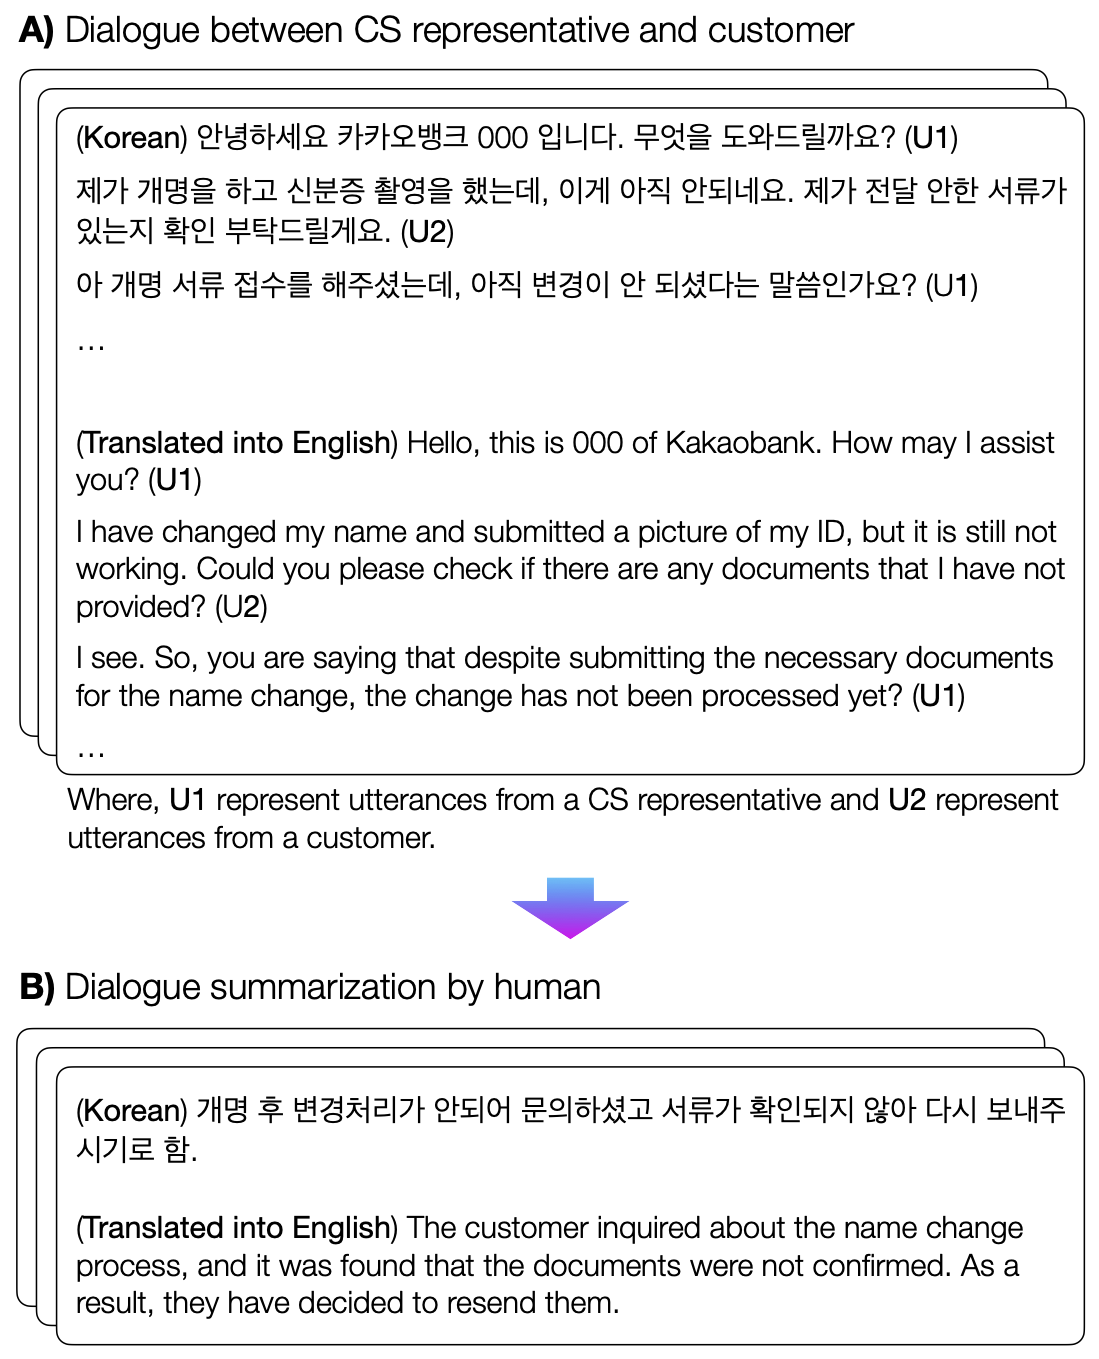
\includegraphics[width=0.48\textwidth]{figures/fig_dialogue.png}
  \caption{Example of KakaoBank's CS datasets: A) dialogue between CS representative (U1) and customer (U2), 
  B) dialogue summarization by a human. 
  }
\label{fig_dialogue}
\end{figure}

As of the first quarter of 2023, KakaoBank serves around 21.2 million customers, accounting for 73\% of the working population in South Korea (\url{https://eng.kakaobank.com}). KakaoBank's services include fee-based banking, such as deposits, loans, and debit cards, as well as platform-related businesses like cobranded credit cards, loan referrals, securities brokerage, and advertising. KakaoBank handles a significant volume of transactions, reaching 4.8 billion in 2022. Operating as an internet-only bank, customer inquiries are directed to a dedicated CSC, which handles an average of 15,000 CS calls daily. After the completion of the CS calls, the CS representatives are responsible for organizing the key customer complaints from the dialogues with clients and summarizing how they were resolved. Additionally, they must identify the specific area of the complaint or inquiry, such as deposits, loans, remittances, or debit cards, and select the appropriate category for logging into the system to finalize the CSC process. 


The objective of this study is to improve the efficiency of various tasks within CSCs by fine-tuning a PLM using a dataset acquired from KakaoBank's CSC. To the best of our knowledge, this is the first research endeavor in the financial sector's CSC to apply generative AI to enhance operational efficiency. In summary, the following contributions were made. First, we developed a language model that can effectively summarize CS dialogues. This was achieved by fine-tuning a Korean PLM model with a few billion parameters using KakaoBank's CSC data. Second, considering the potential impact of the contents in the instruct dataset on the model's performance, we conducted experiments to evaluate the summarization capabilities of the model. Specifically, we investigated how effectively the fine-tuned model (FTM) could summarize CS dialogues when trained solely based on the CS representatives's utterances (Fig.~\ref{fig_dialogue}B) and the entire CS dialogue along with the summaries (Fig.~\ref{fig_dialogue}C) compared with that of the FTM trained with the  KoAlpaca dataset (Fig.~\ref{fig_dialogue}A). 



\begin{figure}[t!]
  \centering
  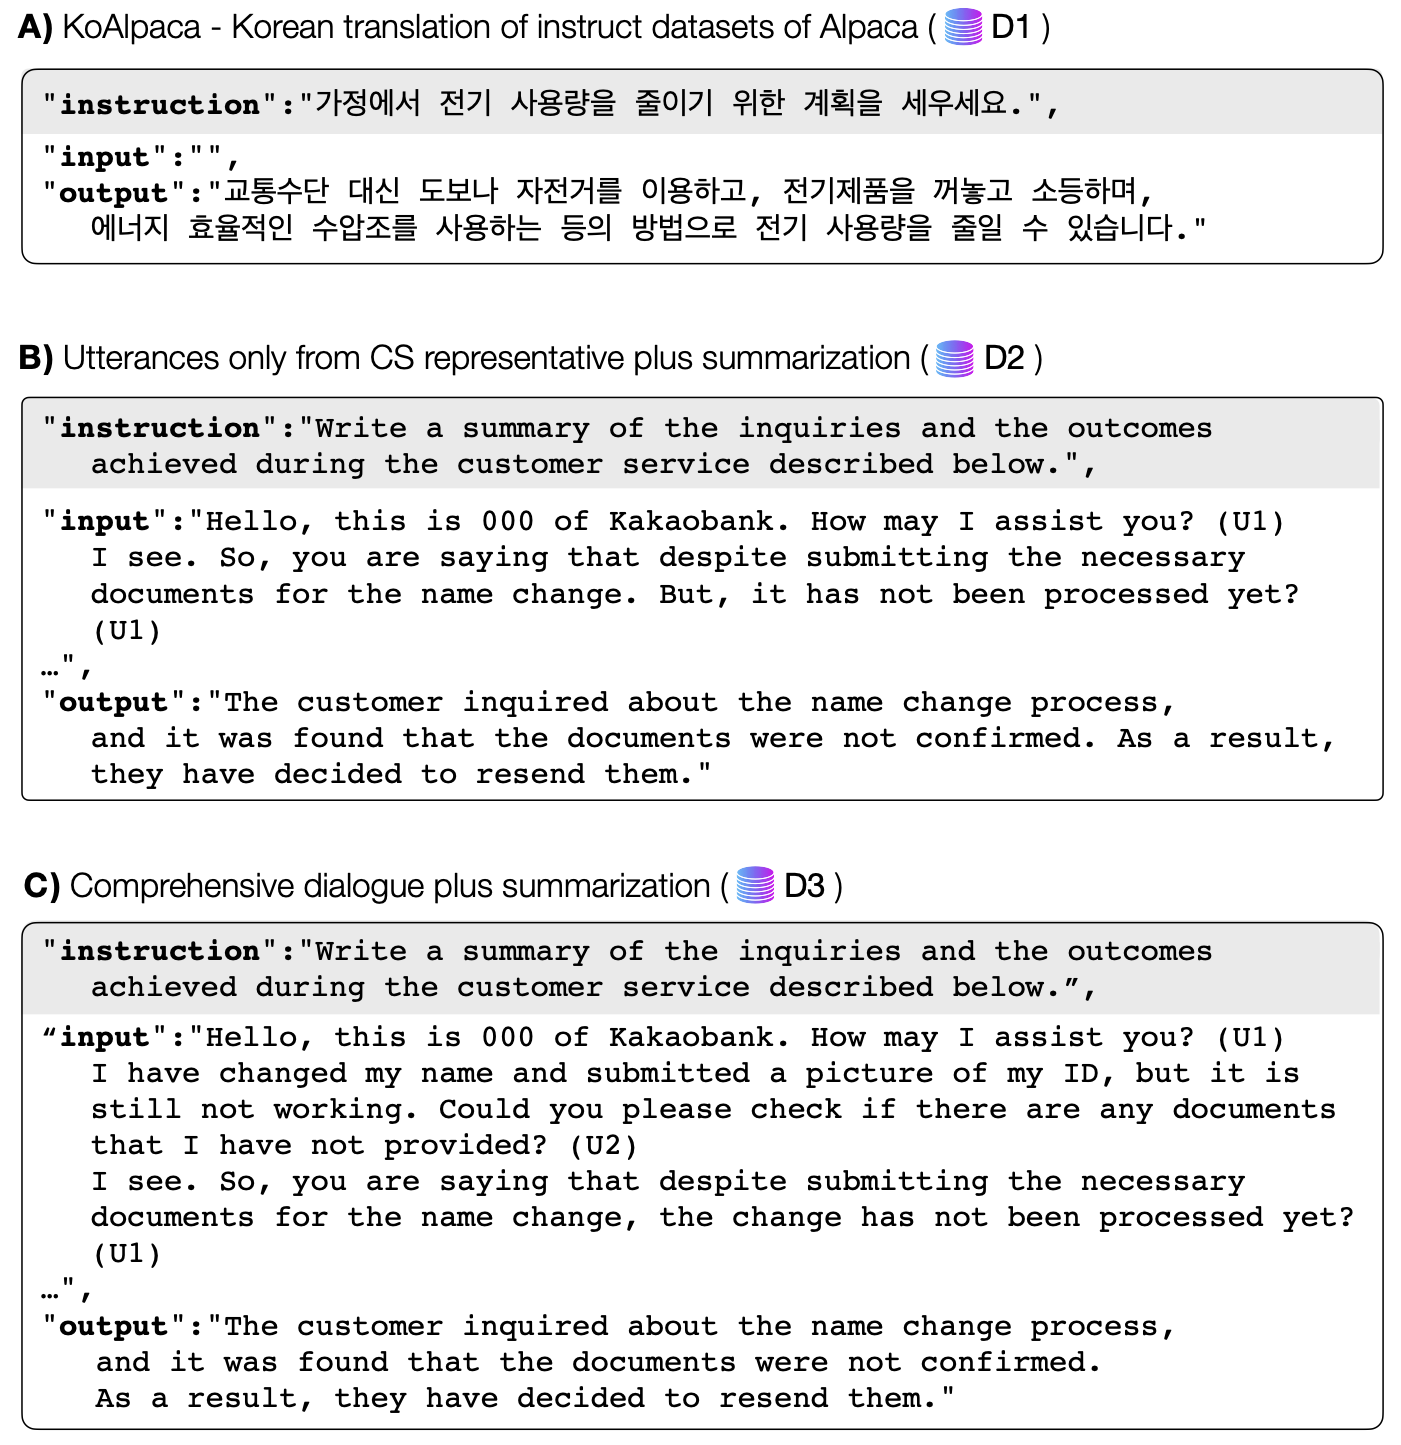
\includegraphics[width=0.48\textwidth]{figures/fig_dataset.png}
  \caption{Example of instruct datasets: 
  A) KoAlpaca instruct datasets that are Korean translations of instruct datasets of Alpaca (D1), 
  B) Instruct datasets with inputs as utterances only from CS representatives (finds U1 sentences in Fig.~\ref{fig_dialogue}A) and outputs as dialogue summarization (D2), 
  C) Instruct datasets with inputs as whole dialogue (finds U1 and U2 sentences in Fig.~\ref{fig_dialogue}A) between CS representatives and customer and outputs as dialogue summarization (D3).
  }
\label{fig_dataset}
\end{figure}



The remainder of this paper is organized as follows: Section~\ref{related_work} presents a comprehensive review of the relevant literature. In Section~\ref{methodology}, the proposed methodology is outlined, including a description of the Korean baseline model and the fine-tuning process using instruct datasets. Section~\ref{evaluation_metrics} describes the evaluation framework of the fine-tuned Korean PLMs. The experimental setups and results are then presented in Sections~\ref{experiments} and \ref{results}, respectively. Finally, Section~\ref{conclusions} summarizes the findings.



\section{Related Works}\label{related_work}
PLMs represent a crucial technology in the realm of AI, which is essential for solving a wide array of downstream tasks. Notably, PLMs with an extensive number of parameters, such as GPT-3~\cite{brown2020gpt3}, PaLM~\cite{chowdhery2022palm}, and OPT~\cite{zhang2022opt}, exhibit remarkable performance across various general-purpose tasks. However, their training has predominantly relies on knowledge-based resources, such as books, web documents, and academic papers, and inadequately incorporates data derived from private conversations between individuals~\cite{gliwa2019samsum,zhong2021qmsum}.


Furthermore, no instances in which PLMs have been trained on conversational data involving interactions between CS representatives and clients have been identified. Nonetherless, several studies have explored the impact of generative AI on chat-based CS operations, investigated fine-tuning techniques that utilize human feedback, and examined prompt-tuning approches aimed at summarizing conversational content. 


\subsection{AI-powered CS center}  
CS operations are vital as a gateway for resolving customer inquiries and concerns, which significantly impacts a company's reputation. Although most CS representatives undergo training to interact with customers based on predetermined guidelines and procedures, substantial variation in productivity exists among them~\cite{syverson:2011}. Efforts have been made to leverage the AI assistants to facilitate more efficient handling of these CS tasks. In one study, a generative AI model was fine-tuned based on actual chat conversations involving approximately 5,000 CS representatives, and its application within a CS system was investigated~\cite{brynjolfsson2023generative}. The findings revealed that AI considerably aided low-skilled workers in improving their task performance and elevating their ability to engage in chat-based CS tasks. In particular, employees in the low-skill group exhibited significant improvements in their ability to engage in chat conversations, reaching levels comparable to those of high-skill employees when using AI assistants. However, it was observed that skilled workers, who were already proficient in their tasks, experienced positive effects in terms of chat volume per hour but did not demonstrate improvements in average handle time~\cite{brynjolfsson2023generative}.




\subsection{Fine-tuning}
Generative AI models encounter persistent challenges when generating harmful or toxic content. To address this issue, researchers have explored the utilization of instruction-tuning techniques with human feedbacks~\cite{ouyang2022training} or machine-generated datasets~\cite{peng2023instruction, wang2023selfinstruct}. Acknowledging the limitations of large-scale language models, such as GPT-3, which has over 100 billion parameters and may struggle with specific tasks such as mathematical problem-solving, a recent study investigated the fine-tuning of an LLaMA baseline model using specialized datasets designed for proficient mathematical problem-solving~\cite{liu2023goat}. Their findings showed an exceptional performance that surpassed existing large language models, particularly in operations involving large numbers, such as addition and subtraction~\cite{liu2023goat}. 


Furthermore, researchers found that fine-tuning language models using instruction datasets significantly enhances their ability to effectively perform unfamiliar tasks, even without prior exposure to them~\cite{wei2022finetuned}. To enhance sentiment classification performance in the finance domain, researchers applied the fine-tuning methodology using a domain-specific corpus~\cite{araci2019finbert}. In contrast, the effectiveness of fine-tuning using imitation datasets was experimentally examined and found to be ineffective in enhancing model performance. Furthermore, fine-tuning using imitation datasets showed subpar performance even in specific downstream tasks~\cite{gudibande2023false}. These results emphasize the significance of fine-tuning using high-quality real-world datasets.




\subsection{Conversation summarization}
During the process of summarizing conversational content, the generation of prompts is vital in  determining result stability, as it can lead to unstable outcomes characterized by factual inconsistencies and hallucinations~\cite{maynez-etal-2020-faithfulness, ladhak-etal-2022-faithful, huang2023}. To address these challenges, one study introduced few-shot learning into GPT-3-based models~\cite{Prodan2022}. By employing an evaluation system rooted in the dialogue structure, researchers enhanced the performance of abstractive summarization through prompt tuning based on high-scoring conversations. Another study applied meta-transfer learning to perform an abstractive summarization task~\cite{Chen_Shuai_2021}. The other study employed the transformation of nondialogue ({\it i.e.}, document) data to bolster the effectiveness of dialogue summarization models~\cite{park-etal-2022-leveraging}. Although studies on abstractive summarization exist, research specifically targeting language models tailored to summarizing CSC within the context of financial domains (Fig.~\ref{fig_dialogue}) is lacking.



\section{Methodology}\label{methodology}
This section describes the characteristics of the baseline PLM and the details of the fine-tuning methodology.


\subsection{Baseline model}
This study aims to develop a fine-tuned language model that can effectively summarize dialogues between clients and CS representatives. For this purpose, we chose the open-source-based Polyglot-Ko as our baseline model owing to its strong performance in Korean. Polyglot-Ko models were specifically designed for the Korean language. They were developed and trained by the EleutherAI polyglot team~\cite{polyglot-ko:2022,polyglot-ko2023note} and trained by using a vast dataset of 863~GB of Korean text (1.2~TB before preprocessing) obtained from TUNiB~(\url{https://tunib.ai}). The datasets consisted of Korean text data from various sources, including blog posts, news articles, fictional texts, patents, questions and answers, and Wikipedia. The Polyglot-Ko models were prepared in four different sizes: 1.3B, 3.8B, 5.8B, and 12.8B. In this study, we selected the 5.8B model as the baseline and utilized the 12.8B model to assess whether there was any performance enhancement. The Polyglot-Ko (5.8B) model consists of 28 transformer layers with model and feedforward dimensions of 4,096 and 16,384, respectively.


\subsection{Fine-tuning using instruct datasets}
Fine-tuning with instruct datasets is a commonly used approach in recent language research that leverages PLMs to enhance performance on specific downstream tasks. This technique entails the initialization of a pretrained model, such as LLaMA, with extensive linguistic knowledge obtained from a substantial corpus of text data. Subsequently, the model is subjected to further training on instruct datasets tailored to the task or domain at hand. These instruct datasets encompass labeled examples, furnishing explicit guidance to the model for executing the desired task. During the fine-tuning phase, the parameters of the model optimized using techniques such as backpropagation and gradient descent, aligning them more closely with the requirements of the specific task. The utilization of instruct datasets during fine-tuning enables the model to transfer its acquired knowledge from pretraining to the target task, thereby facilitating the capture of task-specific patterns and nuances. By synergistically incorporating both the general linguistic knowledge acquired through pretraining and the task-specific guidance from instruct datasets, fine-tuned models exhibit heightened performance and a more comprehensive contextual understanding, providing valuable implications for downstream AI applications in the realm of finance.



\section{Evaluation Framework}\label{evaluation_metrics}
This section describes the evaluation metrics for assessing the performance of the fine-tuning method using instruct datasets for customer dialogue summarization. We utilized two evaluation metrics: the recall-oriented understudy for gisting evaluation (ROUGE)~\cite{lin2004rouge, ganesan2018rouge} and the reference and document aware semantic score (RDASS)~\cite{lee2020rdass}. In text summarization, two factors play a pivotal role: 1) effective selection of content that involves choosing the key information from the document and 2) accurate representation of the same meaning using different expressions ({\it i.e.}, paraphrasing). Although ROUGE is widely used as an evaluation metric for text summarization models, it has limitations in capturing the essence of the summary because it compares the similarity between expert-crafted reference summaries and model-generated sentences. In contrast, RDASS is a comprehensive evaluation metric that considers the relationships among the original document, reference summary, and model-generated summary. Compared to ROUGE, RDASS performed better in terms of relevance, consistency, and fluency of sentences in Korean. Therefore, we employed both ROUGE and RDASS as evaluation metrics, considering their respective strengths and weaknesses of each metric. The mathematical description of each metric is as follows:


\begin{figure}[t!]
  \centering
  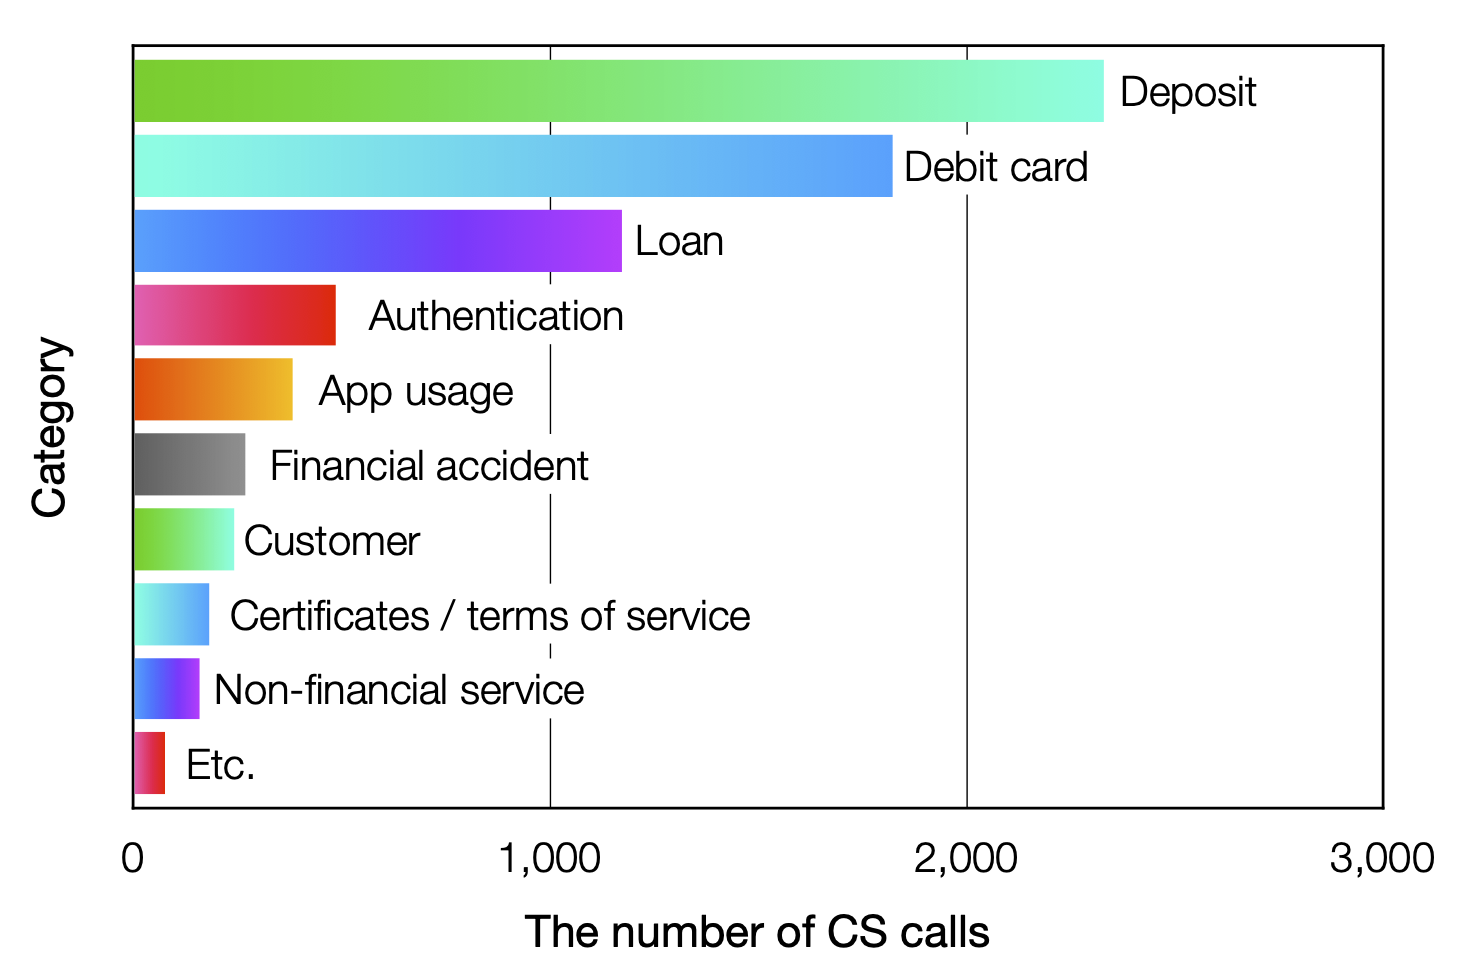
\includegraphics[width=0.48\textwidth]{./figures/fig_cs_category.png}
  \caption{Number of CS calls in each CS category. 
  }
\label{fig_cs_category}
\end{figure}



\begin{figure}[t!]
  \centering
  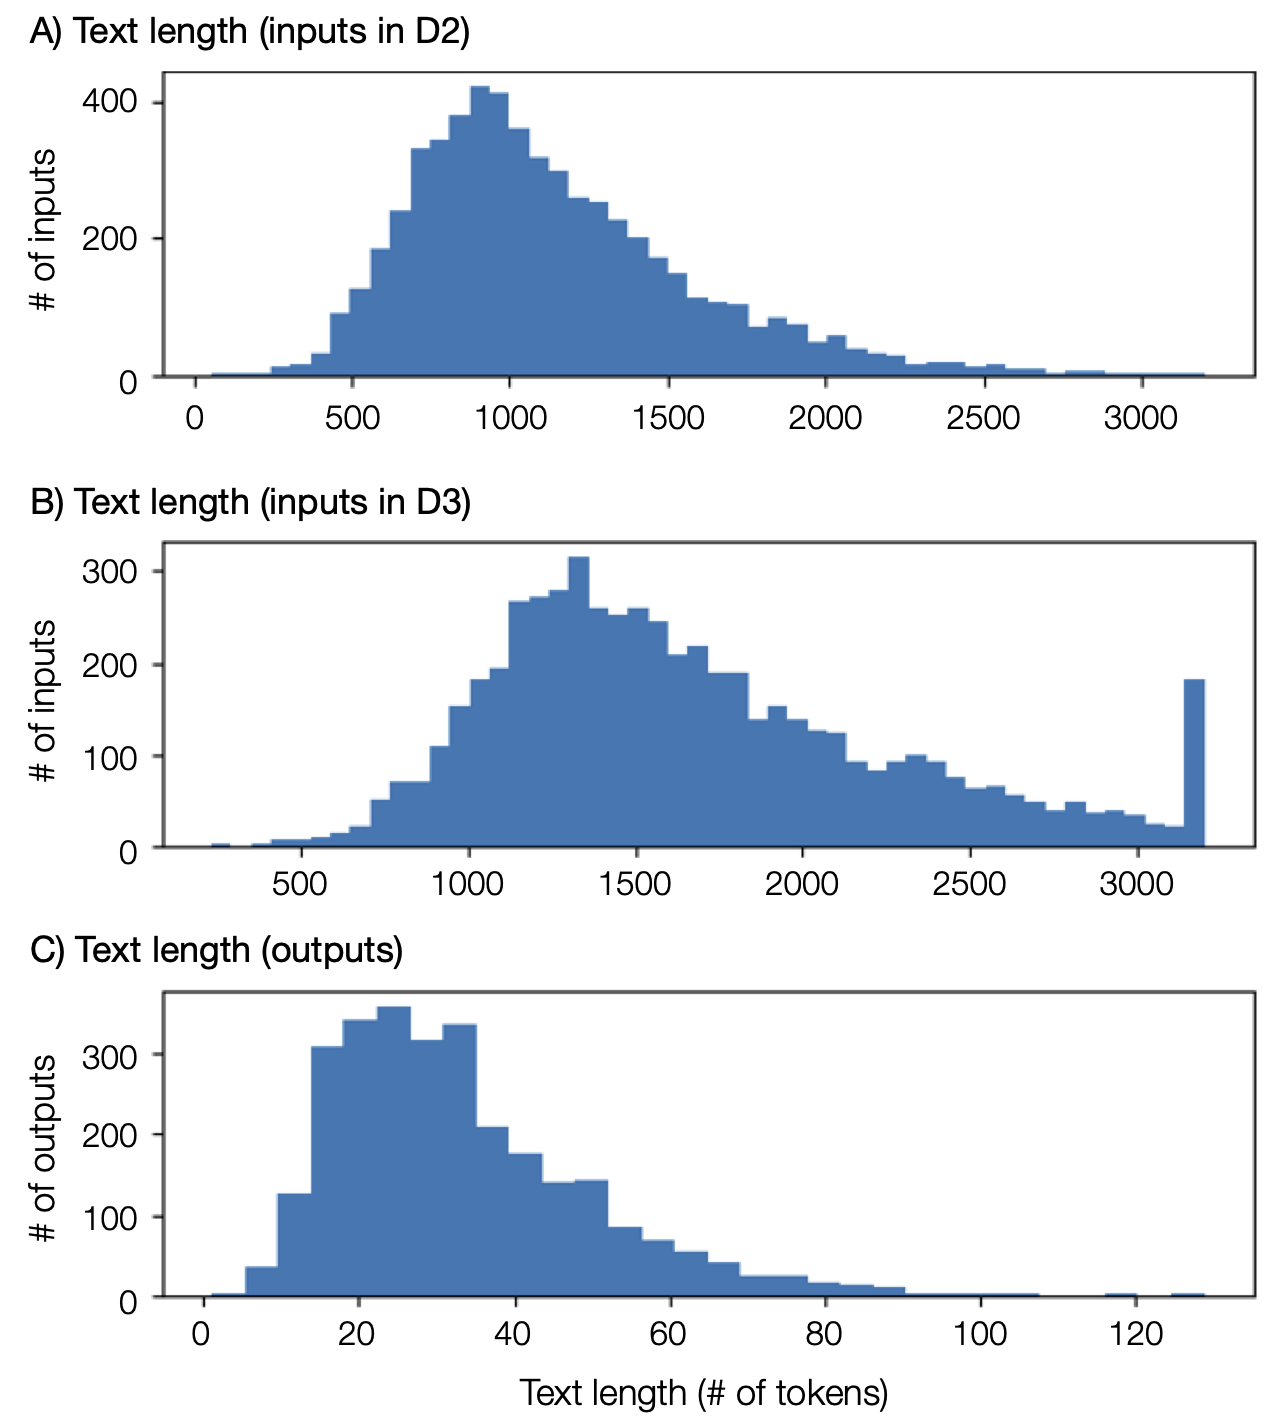
\includegraphics[width=0.48\textwidth]{figures/fig_txtlen.png}
  % 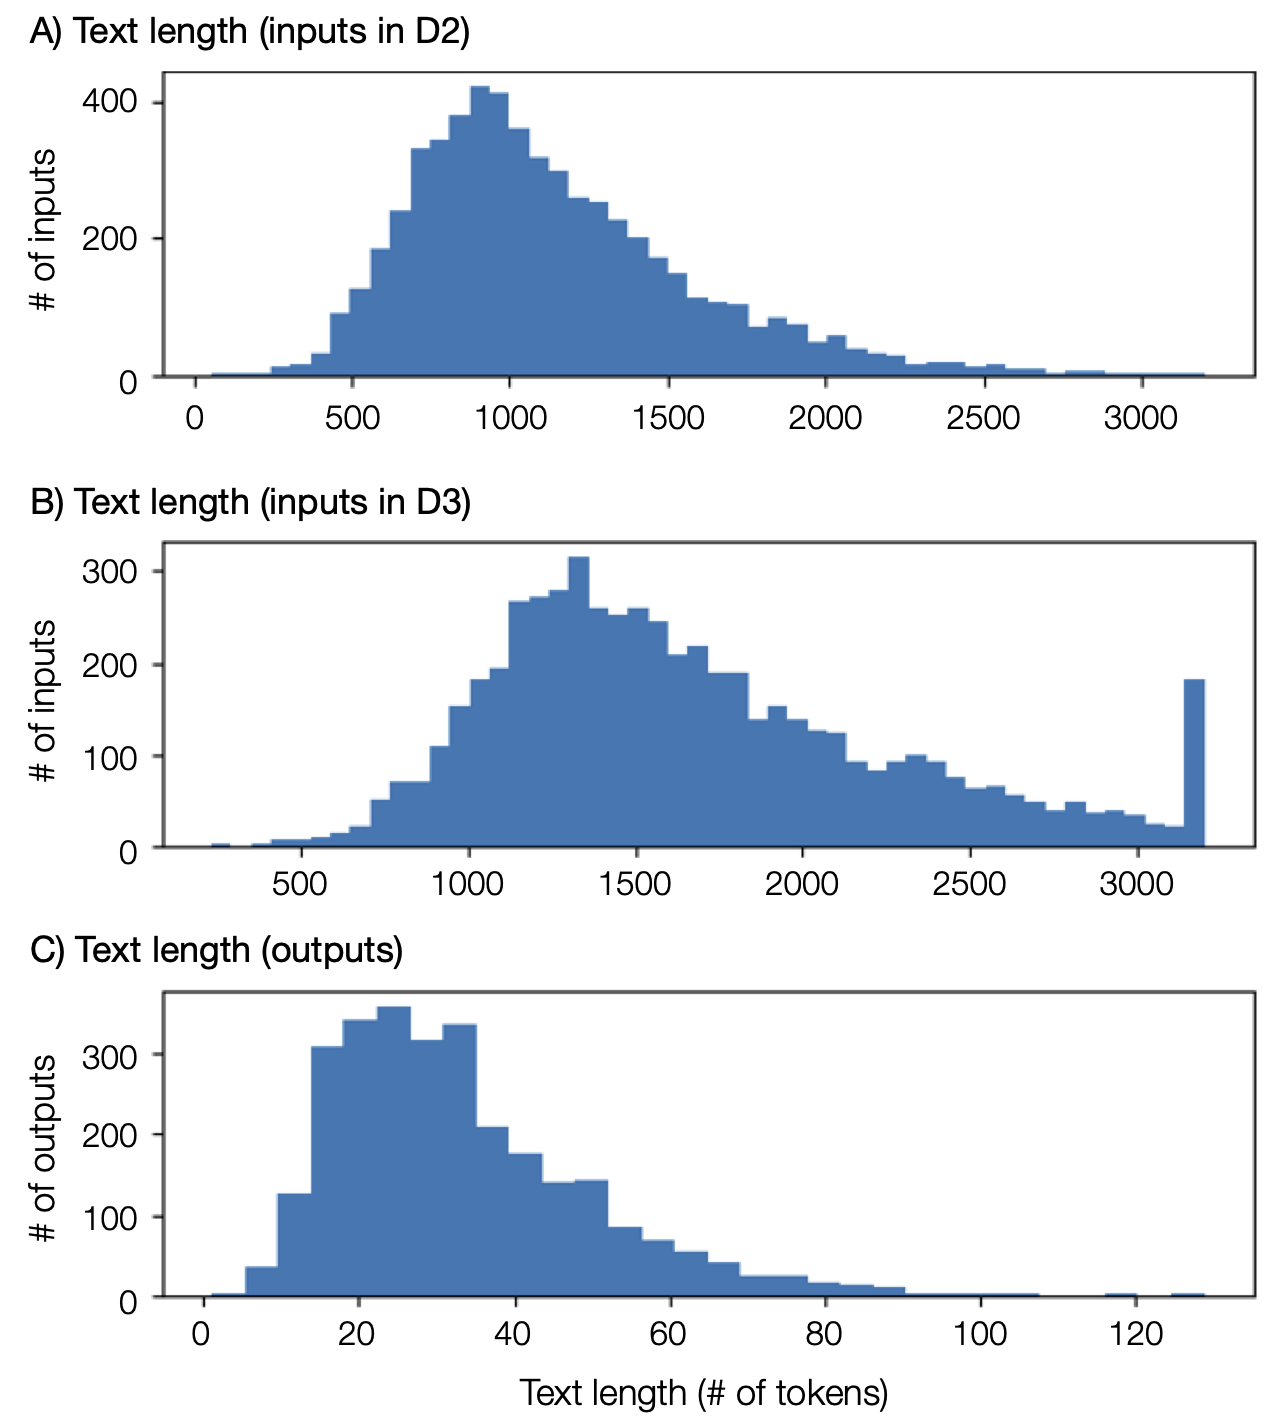
\includegraphics{./figures/fig_txtlen.png}
  \caption{Distributions of the text length in the instruct datasets of KakaoBank's CSC for (A) inputs in D1, (B) inputs in D2, and (C) outputs.
  }
\label{fig_txtlen}
\end{figure}


\subsection{ROUGE} 
ROUGE-N can be computed as the overlap of n-grams between the generated summary and reference summary. Specifically, ROUGE-1 can be computed as the overlap of unigram (each word) between a generated summary and reference summary and is used to assess the quality of automatic summarization systems. In addition, ROUGE-2 can be computed as the overlap of bigrams (pairs of consecutive words) between a generated summary and reference summary and is also used to assess the quality of automatic summarization systems.

ROUGE-L is an evaluation metric that calculates the longest common subsequence (LCS) between a generated summary and reference summary, which captures the overall content overlap and order of words. It is also commonly used to assess the quality of automatic summarization systems.

\subsection{RDASS} RDASS measures the similarity between the vectors of the original document and reference summary. Moreover, it measures the similarity between the vectors of the original document and generated summary. Finally, RDASS can be obtained by computing their average.



\section{Experiments}\label{experiments}
This section provides an overview of the experimental setup, which encompasses various components, such as the preparation of instruct datasets and the development and evaluation of fine-tuned PLMs.




\begin{figure}[t!]
  \centering
  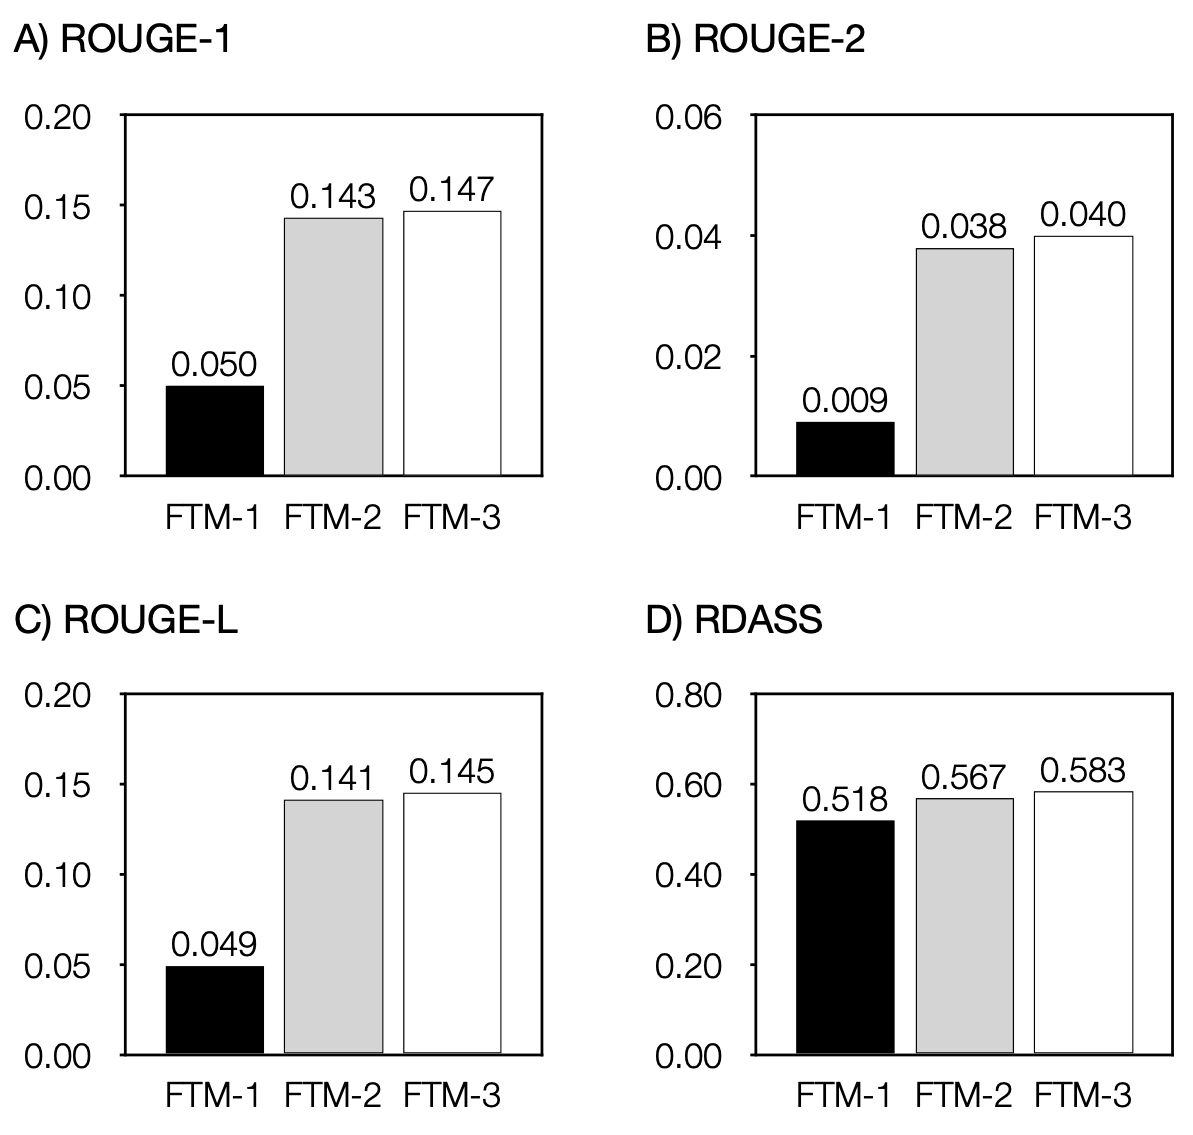
\includegraphics[width=0.48\textwidth]{figures/fig_metrics.png}
  \caption{Summary of model performance experimented through three major fine-tuning models (FTMs): FTM-1 represents fine-tuning Polyglot-Ko (5.8B) using the Koalpaca instruct datasets (see D1 in Fig.~\ref{fig_dataset}); FTM-2 represents fine-tuning Polyglot-Ko (5.8B) using the instruct datasets composed of the utterances of CS representatives and summarization (see D2 in Fig.~\ref{fig_dataset}); FTM-3 represents fine-tuning Polyglot-Ko (5.8B) using the instruct datasets composed of the comprehensive dialogues and summarization (see D3 in Fig.~\ref{fig_dataset}). 
  }
\label{fig_metrics}
\end{figure}


\subsection{KoAlpaca dataset}
The KoAlpaca dataset is a translation of instruction-following data employed to fine-tune the Alpaca model, which is based on the LLaMA model~\cite{alpaca}. It consists of 52K instruction-following instances organized in a JSON file and structured as a list of dictionaries (Fig.~\ref{fig_dataset}). Within each dictionary, three keys, namely instruction,  input, and  output, are associated with string values. The instruction entails comprehensive task descriptions for guiding the model's task, resulting in 52K distinct instructions. The input exhibits variable content that potentially contains the value of an empty string. Finally, the output corresponds to the instruction's answer generated using the utilization of the text-davinci-003 model.




\subsection{KakaoBank's CSC dataset}
In this study, we used a subset of KakaoBank's CS telephone inquiries dataset. We examined the daily CS records in October 2020 and selected a day characterized by a lack of concentrated inquiries on a specific CS category. The audio data was manually transcribed into text, with sensitive information masked for privacy. The CS engagements covered various topics, including financial services (deposits, debit cards, loans) and other areas like authentication, app usage, and financial accidents. Fig.~\ref{fig_dialogue}A shows an example of a CS dialogue exchange. The CS session typically starts with a salutation and restatement of the customer's inquiry for confirmation. This iterative conversation continues until the CS representative resolves the issue or provides potential solutions. We labeled the data to create instruct datasets for dialogue summarization in CS dialogues. Fig.~\ref{fig_txtlen} depicts the distribution of text lengths for complete dialogues, CS representatives' utterances, and reference summaries.





\begin{figure}[t!]
  \centering
  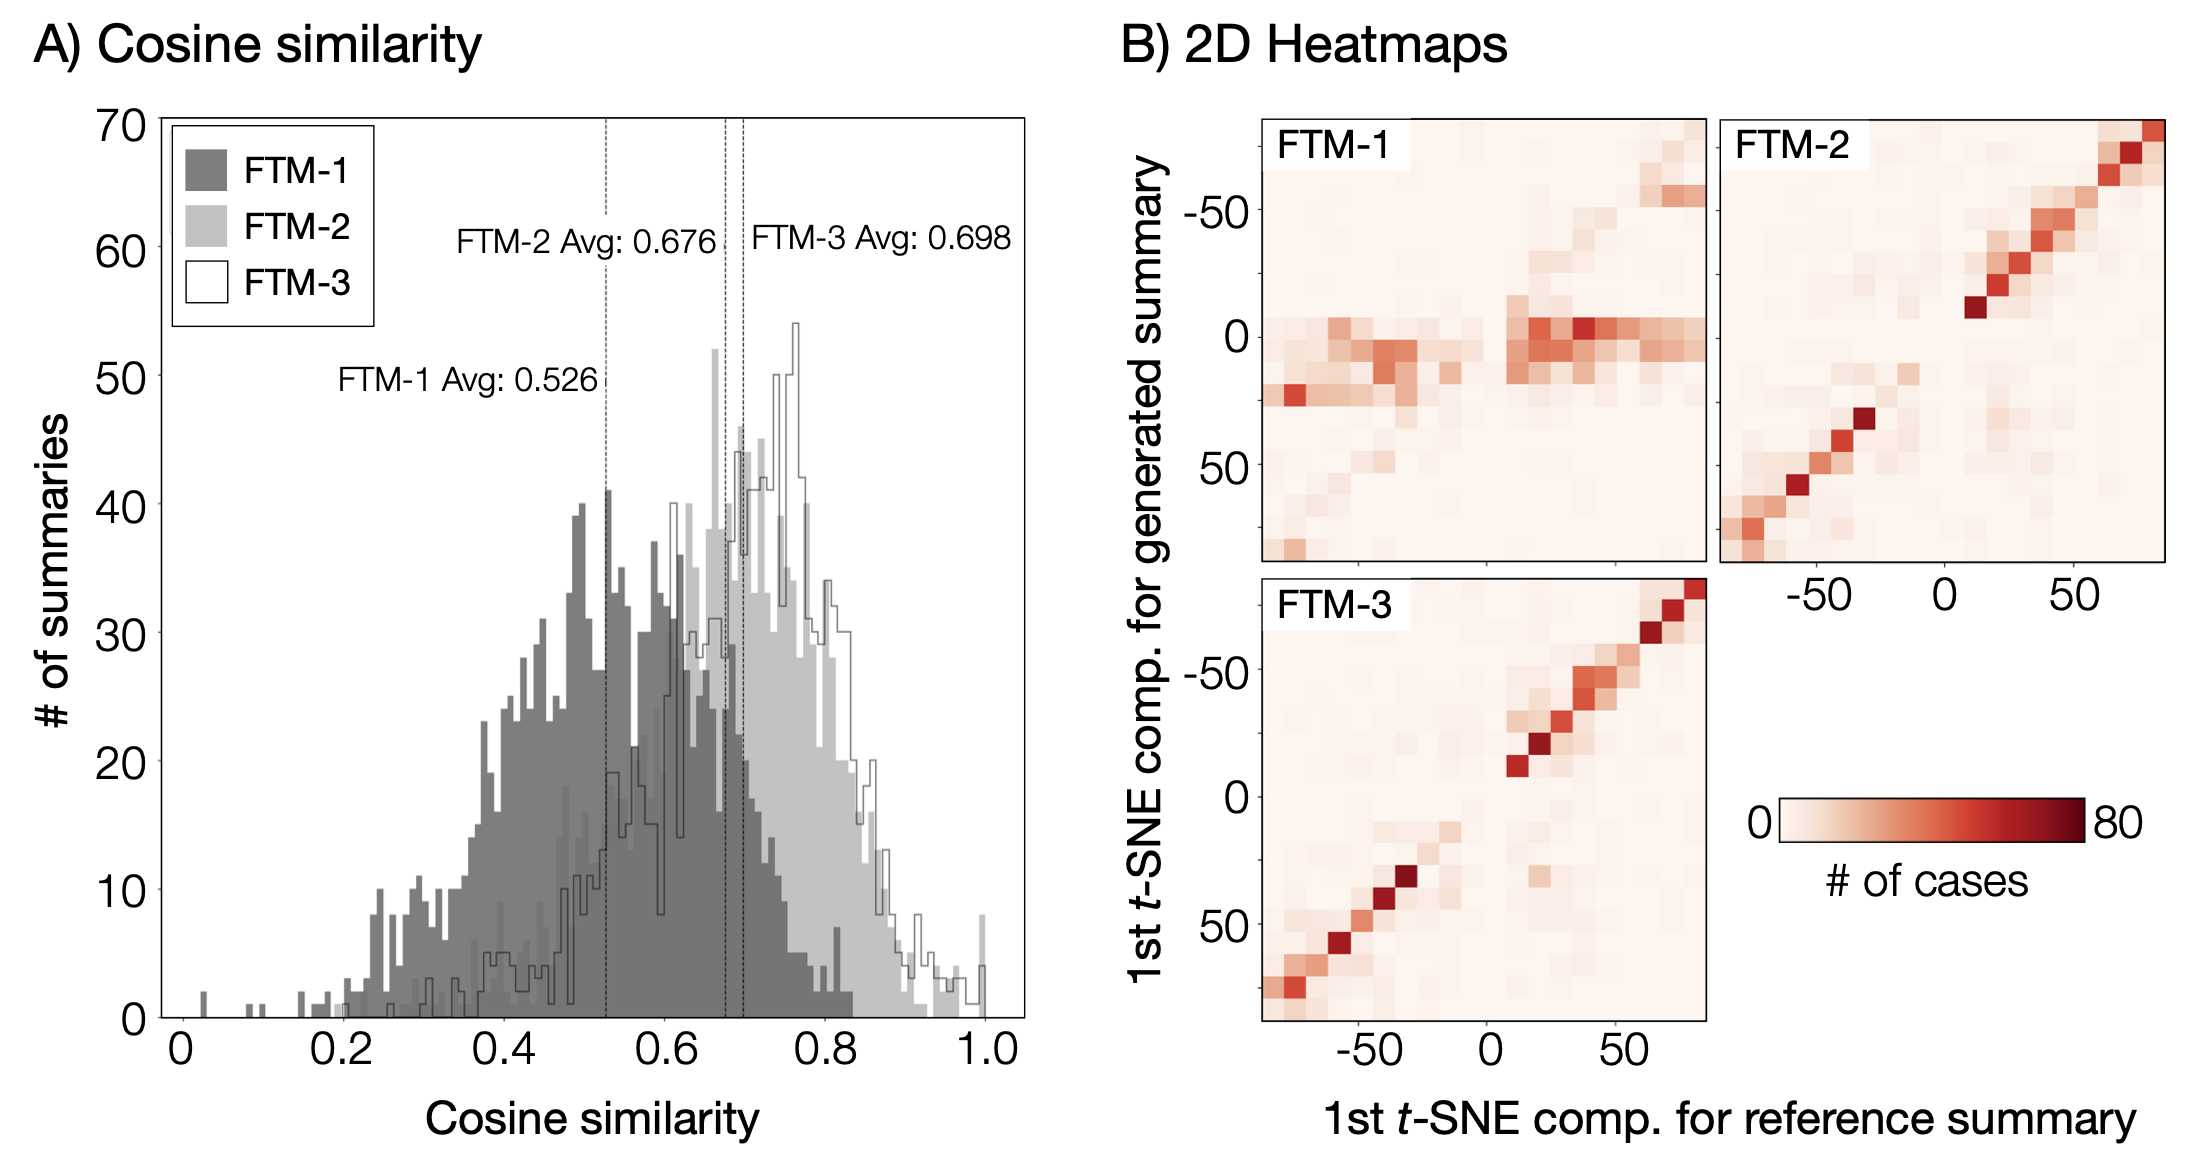
\includegraphics[width=0.48\textwidth]{figures/fig_similarity.png}
  \caption{Similarity measures between the reference and generated summaries. (A) Cosine similarity of the embedding vectors between the reference summaries and the generated summaries. (B) 2D heatmaps of the first component of $t$-SNE between the reference and generated summaries for the fine-tuning model 1 (FTM-1) (top-left), FTM-2 (top-right), and FTM-3 (bottom-left).
  }
\label{fig_similarity}
\end{figure}



\subsection{Fine-tuning training}
We divided the KoAlpaca and KakaoBank's CSC instruct datasets into training and test datasets in a ratio of 8:2, respectively. We then used Polyglot-Ko (5.8B) as the baseline model and performed  fine-tuning using various instruct datasets. The first FTM (FTM-1) involved fine-tuning using KoAlpaca instruct datasets (see Fig.~\ref{fig_dataset}A). This model served as a baseline for evaluating whether a Korean language model trained with general knowledge-based Korean instruct datasets could effectively perform dialogue summarization. The second FTM (FTM-2) involved fine-tuning using the utterances of the CS representatives and summarization (see Fig.~\ref{fig_dataset}B). The third FTM (FTM-3) involved fine-tuning using the entire CS dialogue and summarization (see Fig.~\ref{fig_dataset}C). Furthermore, an additional FTM (FTM-4) was developed by fine-tuning Polyglot-Ko (5.8B) by integrating the KoAlpaca and KakaoBank's CSC instruct datasets.




\subsection{Model performance evaluation}
Each FTM model was subjected to inference procedures on the test dataset, followed by an assessment of the similarity between the reference and generated  summaries using the ROUGE and RDASS metrics. In addition, the cosine similarity of the embedding vectors between the reference and generated summaries was measured to determine which FTM exhibited the best performance. Furthermore, the embedding vectors of the reference and generated summaries were transformed using $t$-distributed stochastic neighbor embedding ($t$-SNE)~\cite{vanDerMaaten2008} and visualized as a 2D heatmap of the first t-SNE component to assess the model's performance. Measurement of certain aspects of the FTM using ROUGE or RDASS proved to be difficult, necessitating the validation of its effectiveness through qualitative methodologies.





\begin{table}[t!]
  \fontsize{8pt}{8pt}\small
  \caption{Examples of the reference and generated summaries using fine-tuning models (FTMs). The customer's situation is highlighted in cyan, whereas the primary inquiry is highlighted in orange within the given context.}

  \begin{tabular}{l p{7.8cm} }
      \toprule 
      \multicolumn{2}{l}{\bf Reference summary} \\  
      & {\color{cyan} Inquired about expediting the process because it was taking time after applying for the removal of the transfer limit}, {\color{orange}Informed about errors in the documents and provided guidance on resubmitting the required documents.}\\
      \midrule 
      \multicolumn{2}{l}{\bf Generated summary by FTM-1}\\ 
      & Because you are registered with an account that has a daily limit.\\
      \midrule 
      \multicolumn{2}{l}{\bf Generated summary by FTM-2}\\
      &  {\color{cyan}Applied the removal of the limit on the account. Requested urgent processing}.\\
      \midrule 
      \multicolumn{2}{l}{\bf Generated summary by FTM-3}\\
      & {\color{cyan} Requested expedited processing because it wasn't being handled after applying for the removal of the transfer limit}. {\color{orange}Provided instructions for document submission and guidance on the process}.\\
      \bottomrule
  \end{tabular}
  \label{table_examples}
\end{table}


\subsection{Multiple instruction templates}\label{sec_multiple_instructions}

To improve the zero-shot ability of the fine-tuned language model~\cite{wei2022finetuned}, we conducted fine-tuning using multiple instructions to enable the versatile utilization of the summarization task. For example, it can be applied to a task involving the detailed summarization of CS inquiries and the resolution process, as well as a task involving the brief summarization task of CS inquiries. To obtain various forms of summarization results for the same CS dialogue, we performed fine-tuning using multiple instruction templates to apply the fine-tuned model to various summarization tasks. Examples of the instruction templates are as follows:

\begin{itemize}
  \item {\bf Instruction 1}: Write a detailed summary of the inquiry and the resolution process in the following CS dialogue.\\
  Additional requirements of instruction 1: The summary must include the specific words and have a token length greater than or equal to 45.
  \item {\bf Instruction 2}: Write a brief summary of the following CS dialogue.\\
  Additional requirements of instruction 2: The summary must include the specific words and have a token length of less than or equal to 25.
  \item {\bf Instruction 3}: Write a short summary of the following CS inquiry within five words.\\
  Additional requirements of instruction 3: The summary must not include the specific words and must have a token length between 5 and 15.
\end{itemize}

In the above instructions, the specific words that should and should not be included in the summaries are as follows: guide, answer, progress, closed, emergency, resolved, and completed. 



\section{Experimental Results}\label{results}

In this section, we describe the evaluation results of the FTMs for CS dialogue summarization; we present the ROUGE and RDASS metrics for the various FTMs. Additionally, an assessment of the similarity between the reference and generated summaries by each FTM using cosine similarity and $t$-SNE methods are provided.





\subsection{Performance of fine-tuning models}
The summarization performances of the FTMs were evaluated by using two metrics: ROUGE and RDASS (Fig.~\ref{fig_metrics}). The reference fine-tuning method (FTM-1) yielded ROUGE-1, ROUGE-2, ROUGE-L, and RDASS scores of 0.050, 0.009, 0.049, and 0.518, respectively. Subsequently, the FTM-2  demonstrated improved performance, with ROUGE-1, ROUGE-2, ROUGE-L, and RDASS scores of 0.143, 0.038, 0.141, and 0.567, respectively. FTM-3 showed further enhancement, with ROUGE-1, ROUGE-2, ROUGE-L, and RDASS scores of 0.147, 0.040, 0.145, and 0.583, respectively. Among the three major FTMs, fine-tuning by incorporating comprehensive dialogue data and summarization delivered the most favorable outcomes.

 

We visually explored the summaries generated by the FTMs compared to the reference summaries (Table~\ref{table_examples}). FTM-1 produced a summary unrelated to the reference, while FTM-2 partially contained essential details. FTM-3, although slightly different, concisely summarized the customer's inquiry and the CS representative's guidance, closely aligned with the reference summary. Lee {\it et al.} (2021) reported that training a masked language model (MLM) with financial domain data led to an approximate enhancement of 3.3\% in ROUGE-1 and 5.7\% in ROUGE-L compared to the absence of nonfinancial data~\cite{lee2021optimizing}. This observation implies that training substantial knowledge in the financial domain is imperative for achieving commendable performance in document summarization tasks within the financial context. Our research findings are in line with those of  previous research, indicating that higher performance on a summarization task in the financial domain necessitates training models with appropriate financial data. 



To investigate the hypothesis regarding the potential improvement in FTM performance through training with multiple sources of instruct datasets, additional experiments were conducted. The evaluation of the summarization performance for the model trained using fine-tuning with both the dialogue and KoAlpaca instruct datasets (FTM-4) resulted in ROUGE-1, ROUGE-2, ROUGE-L, and RDASS scores of 0.136,   0.035, 0.133, and 0.576, respectively. Nevertheless, these results revealed a lower performance compared with FTM-3, which was trained solely using the dialogue instruct dataset. Specifically, FTM-4 demonstrated a decrease in performance relative to FTM-3, with reductions of 7.6\%, 14.6\%, 8.1\%, and 1.1\% in ROUGE-1, ROUGE-2, ROUGE-L, and RDASS, respectively. These findings indicate that task-specific instruct datasets have a beneficial effect on enhancing the performance in fine-tuning for specific downstream tasks. However, the inclusion of a substantial number of instruct datasets unrelated to the task can have a detrimental effect on the model's performance.


Finally, additional experiments were conducted to examined the impact of the baseline model size on the performance of the downstream task of dialogue summarization. In this study, instruct datasets identical to those used in FTM-3 were employed, with a modification of the baseline model to Polyglot-Ko (12.8B) for fine-tuning training (FTM-5). A performance evaluation was conducted using the ROUGE and RDASS metrics. FTM-5 model exhibited performance scores of 0.149, 0.042, 0.148, and 0.584 for ROUGE-1, ROUGE-2, ROUGE-L, and RDASS, respectively. Compared to FTM-3, these values displayed improvements of 1.8\%, 4.4\%, 1.9\%, and 0.1\% for ROUGE-1, ROUGE-2, ROUGE-L and RDASS, respectively. This observation highlights that larger parameters in the baseline PLM can help improve the performance in the dialogue summarization task. 




\begin{figure}[t!]
  \centering
  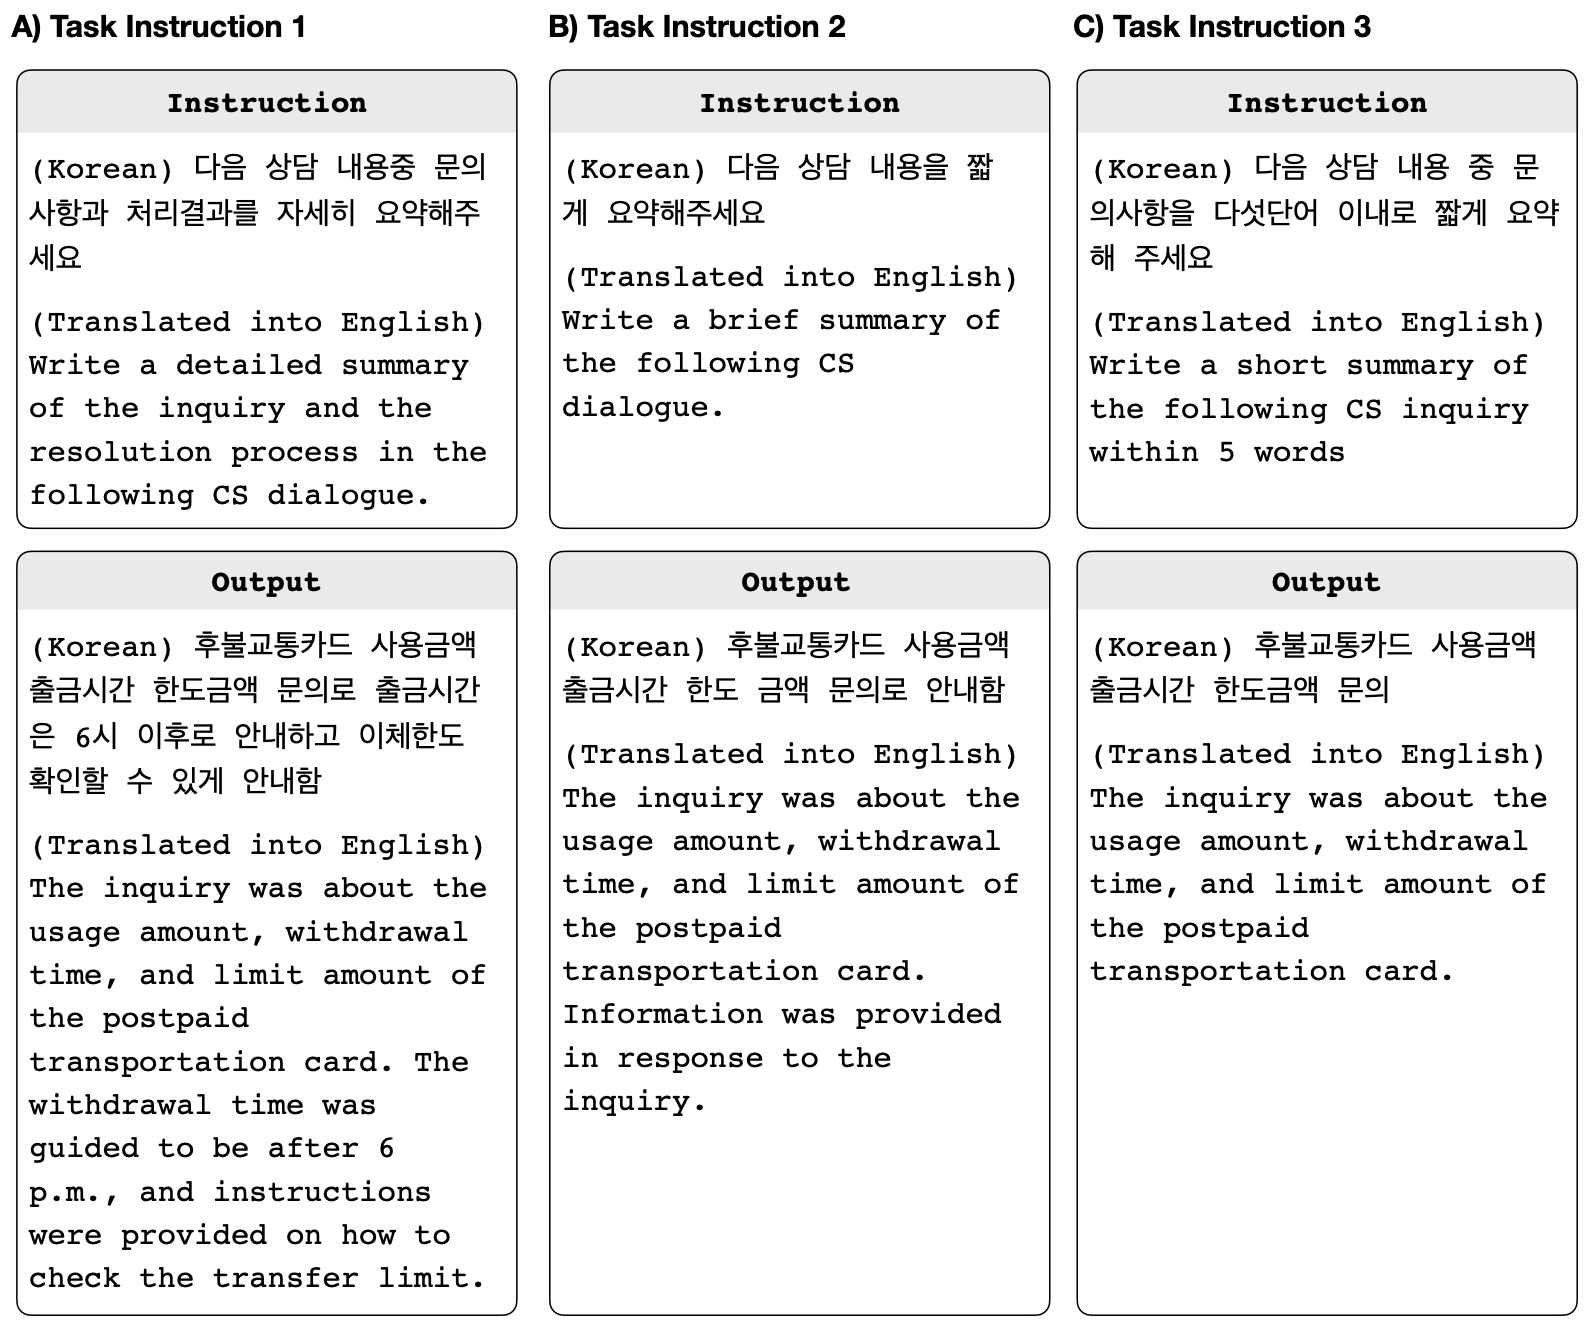
\includegraphics[width=0.48\textwidth]{./figures/fig_var_tasks.png}
  \caption{Illustrative inference outcomes of the fine-tuning model using multiple instruction templates. The task instructions and their corresponding outputs are demonstrated for (A) an instance of instruction 1 (Write a detailed summary of the inquiry and the resolution process in the following CS dialogue), (B) instruction 2 (Write a brief summary of the following CS dialogue), and (C) instruction 3 (Write a short summary of the following CS inquiry within 5 words). 
  }
\label{fig_var_tasks}
\end{figure}




\subsection{Similarity measures}
To assess the quality of generated summaries by the FTMs, we evaluated the cosine similarity of the embedding vectors between the reference summaries produced by humans and the generated summaries produced by the FTMs. As illustrated in Fig.~\ref{fig_similarity}A, the average cosine similarity values of the embedding vectors between the reference and generated summaries by FTM-1, FTM-2, and FTM-3 are 0.526, 0.676, and 0.698, respectively.


Additionally, we projected the embedding vectors of the summaries onto $t$-SNE and visualized the 2D heatmaps depicting the first $t$-SNE components alongside the reference and generated summaries (Fig.~\ref{fig_similarity}B). Within the 2D heatmap, an elevated value in the diagonal bins indicates a heightened degree of similarity between the sentences of the reference and generated summaries. Conversely, a higher value in the off-diagonal bins implies a reduced level of similarity between the sentences of the reference and generated summaries. Specifically, in the case of FTM-1, the off-diagonal bins are predominantly populated, indicating a lower degree of similarity between the generated and reference summaries. Conversely, for FTM-2 and FTM-3, the distribution tends to concentrate more within the diagonal bins, suggesting a greater similarity between the generated and  reference summaries. Notably, FTM-3 exhibits values in the off-diagonal bins that are closer to 0 compared to FTM-2, which suggests that the sentences of the generated summaries by FTM-3 are most similar to the reference summaries.






\subsection{Fine-tuning with multiple instruction templates}
Examples of inference results of zero-shot unseen data for the fine-tuning using multiple instruction templates, which are composed of three different types based on the length of the summary and whether specific words (see Section~\ref{sec_multiple_instructions}) are included in the summary, are shown in Fig.~\ref{fig_var_tasks}. Fine-tuning using a single instruction template produces almost similar outputs ({\it i.e.}, similarly generate summaries) even if various instructions are given during inference. However, fine-tuning using multiple instruction templates obtains different outputs depending on the instruction during inference. Specifically, Instruction 1 generated a detailed summary, whereas Instruction 2 produced a more concise summary. Instruction 5 provided a summary in five Korean words. Although it was expanded to more than five words during the translation process into English, it performed well in Korean in terms of the task. 




\section{Conclusions}\label{conclusions}
Although GPT-3 has features such as multilingual support, there are several constraints to consider when applying it to solving specific business problems that aligns with the culture, policies, and regulations of each country. In this study, we proposed a method for addressing the downstream task of dialogue summarization by fine-tuning using real-world instruct datasets. We developed a reference FTM using Polyglot-Ko (5.8B) as the baseline PLM and the KoAlpaca instruct dataset containing various zero-shot and partially document summarization instructions. We compared this model with the FTM-3, which was fine-tuned using KakaoBank's CS dialogues and summarization as the instruct dataset. The results demonstrated that FTM-3 based on KakaoBank's internal datasets outperformed the reference model, showing a 199\% and 12\% improvement in ROUGE-L and RDASS, respectively.


Typically, the tasks of CS representatives are well-documented in the form of guidelines. For example, detailed explanations of financial products, methods of consultation or customer interaction, ways to summarize and condense content after CS calls, and methods of selecting CS categories are often organized in documents to ensure that employees are well-versed. However, tasks such as addressing customer complaints or summarizing CS records rely heavily on individual skills, even when following guidelines. Automating these areas of work was deemed infeasible until the advent of generative AI~\cite{polanyi:1966}, which can memorize detailed product explanations, engage in conversations by following predefined guidelines, and effectively extract key points for summarization. By utilizing a fine-tuned language model to summarize CS dialogues, we anticipate a certain level of standardization in summarization tasks between high- and low-skilled workers. 


In this study, we developed a model that summarizes customer inquiries received through telephone calls. However, this model could be expanded to summarize chat-based CS inquiries or iterative email-based CS inquiries. Furthermore, by fine-tuning using different instructions, such as 1) simply summarizing the dialogue and 2) summarizing the dialogue in five words, it can be extended to categorize CS types. Our approaches can be applied to the CS operations of most financial institutions targeting retail customers.


In conclusion, this study highlights the importance of task-specific fine-tuning using appropriate instruct datasets to achieve effective performance in specific downstream tasks. We suggest that fine-tuning using real-world instruct datasets is a powerful and cost-effective technique for developing generative AI in the business domain.



%% Print the bibliography
% \printbibliography

\bibliography{references.bib} 



\end{document}
\endinput
%%
%% End of file `sample-sigconf.tex'.
